\documentclass{article}
\usepackage{setspace}
\usepackage{listings}
\usepackage{float}
\usepackage{amssymb,amsmath}
\usepackage{wrapfig}
\usepackage{url}
\usepackage{graphicx}
\usepackage{fancyvrb}
\usepackage{mathtools}
\usepackage{floatflt}
\usepackage{framed}
\usepackage[square,sort,comma,numbers]{natbib}
\usepackage[margin=1in]{geometry}
\doublespacing
\title{The Count Distinct Problem}
\author{Steven Rosendahl}
\date{}
\begin{document}
\maketitle
\indent Processing data efficiently has always been a goal of organizations that collect data; companies like Facebook and Google have been collecting and storing data for as long as they have existed.
One important statistic that is useful to companies is the number of distinct elements in a large set of data.
The question of how many distinct elements there are in a given set is called the \textit{count distinct} problem. 
Several algorithms exist that can solve the count distinct problem; we will consider three of them:
the hash table, the Linear Probabilistic Counter, and the HyperLogLog. 
To analyze these algorithms, we will apply them to real world problems, namely (1) The Pok\'emon Problem, which poses the question ``How many unique Pok\'emon encounters will a player face in a given play through of a game from each generation?'' (2) The Facebook Problem, which asks ``How many unique Facebook app installs are made on any given day?'' and (3) The Twitter Problem, which asks ``how many unique hashtags are created on any given day?''
We use the hash table, the Linear Probabilistic Counter, and the HyperLogLog to solve each problem, respectively.\\

\indent The first solution to the count distinct problem is called a hash table. 
A hash table is a matrix that is stored in memory where each entry is uniquely obtained from another value, called a key. 
The algorithm is as follows:
\begin{center}
Let $\mathbb{S}$ be a set of random elements. In order to count the number of distinct elements in $\mathbb{S}$,
\begin{enumerate}
\item Apply a bijection, $h(n)$ to all $n\in\mathbb{S}$, and store the result in a set $\mathbb{V}$.
\item Count the number of elements in $\mathbb{V}$. $||\mathbb{V}||$ will be the number of unique elements in $\mathbb{S}$.
\end{enumerate}
\end{center}
Since $h$ is a bijection, it is injective. 
As a result, if we take any $x\in\mathbb{S}\ \text{and}\ y\in\mathbb{S}$, then if $x = y$, they will hash to the same value; since we want to know how many distinct values exist in $\mathbb{V}$, we ignore the duplicate values produced by the hash function \cite[p. 6]{Maurer}. 
For example, say we want to count the number of distinct names in the set $\mathbb{S} = \{\text{``Alice''},\text{``Emily''},\text{``Alice''}\}$. 
We create a simple hash function that is bijective for the set $\mathbb{S}$.
Our function will first translate each letter in a word into its corresponding numerical position in the alphabet.
We then sum up the total of each of the numbers (call this $n$), and determine the remainder of division of $n$ and the total number of letter in the name.
Applying our hash function on the first element, ``Alice'', yields $1 + 12 + 9 + 3 + 5 = 30$, which when divided by 5 produces a remainder of 0; therefore ``Alice'' hashes to 0.
When the hash function is passed all the elements of $\mathbb{S}$, we get a set $\mathbb{V} = \{0,4\}$. 
The cardinality, or size, of $\mathbb{V}$ (denoted as $||\mathbb{V}||$) is 2, so there were two distinct elements in $\mathbb{S}$. 
In this example, the hash function we chose was bijective.
However, this may not always be the case. In fact, it is practically impossible to create a hash function that is truly injective for huge amounts of data \cite[p. 6]{Maurer}. 
For smaller sets of data, however, we can create a hash function that is surjective. 
The Pok\'emon  problem provides a good example of the benefits of a hash table.\\

\indent The most beneficial aspect of the hash is that it has a 0\% error rate. 
In other words, the cardinality of $\mathbb{V}$ is exactly the number of distinct elements are in $\mathbb{S}$, assuming the hash function is bijective. 
We know that for very large $\mathbb{S}$, the hash table method is incredibly inefficient, but for the Pok\'emon problem, we are dealing with $\mathbb{S}$ small enough to apply the hash table. 
In this particular case, 721 Pok\'emon  can be encountered \cite{Pokemon}, which means that the maximum size needed for our set $\mathbb{V}$ is 721. 
Typically, a player will encounter in the neighborhood of 1000 wild Pok\'emon a game, and with a total of 6 generations of games, we have a set $\mathbb{S}$ of size 6000. 
The hashing function we created earlier will not be good enough here; instead we can create a new hashing function where we sum up the value of the name as before, then add the Pok\'emon 's unique id, and finally mod that value with 721.
\begin{floatingfigure}[H!]{8cm}
\centering
\begin{framed}
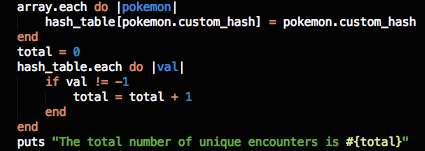
\includegraphics[scale=0.4]{pkmn_problem/hash_01}
\caption{Hashing Pok\'emon based on name and type}
\end{framed}
\end{floatingfigure}
\noindent In order to come up with a set $\mathbb{S}$, we can randomly populate an array with 6000 Pok\'emon; we are assuming that a player has an equal chance to run into any Pok\'emon, and that they can encounter all Pok\'emon more than once.
Running the code in \textit{Figure 1} gives us a final answer of 461 unique encounters with wild Pok\'emon. 
In the case of the Pok\'emon problem, a simple hash function suffices, since the only collisions encountered are Pok\'emon with the same name; we realistically can test the hash function by passing it all 721 Pok\'emon and determining whether or not there are 721 hashed values.
If we consider a larger data set, however, we may not be able to create a bijective hash function.\\

\indent Imagine that we are solving the Twitter problem where we want to count the number of distinct hashtags on Twitter on a given day. 
Our set $\mathbb{S}$ will now contain every hashtag that was made on a given day. 
We know that we want a hash function that is bijective, but this is an unrealistic, since we could have some $x \in \mathbb{S}$ and $y\in\mathbb{S}$ where $x \neq y$ but $h(x) = h(y)$. 
To model this issue, we can consider the following scenario:
\begin{quote}
On October 30th, 2015, Mojang released a special Halloween cape to all players of the popular video game Minecraft. 
As a result, ``\#cape'' began trending on Twitter.
On the same day, Target announced that all their \textit{Bob's Burgers} costumes would be on sale for the low price of \$12.95, and ``\#bob'' began trending on Twitter.
\end{quote}
Our previous hash function will not work in this case, since both ``\#bob'' and ``\#cape'' hash to the same value. 
On a larger scale, such as the Facebook or Twitter problem, we would need to either handle collisions (where two different keys hash to the same value) or create a better hash function. 
Creating a way to handle collisions would not be beneficial, since the data are being processed in real time. 
We would not be able to tell if we were hashing a value we already saw or hashing a new value that happened to hash to the same value as another element we already saw. 
As a result, we would have no way to know which keys were different and which keys were the same when looking at $\mathbb{V}$ \cite[p. 6]{Maurer}. 
Since the collision policy would not help us, we need to come up with a better hashing function.\\

\indent More complex hash functions, such as SHA-2 (Secure Hash Algorithm 2) or MD5 (Message Digest 5), offer a solution to the collision problem. SHA-2 is used by organizations such as the NSA to encrypt data and has yet to produce any collisions when hashing values \cite[p. 301]{SHA-Algo}. However, this is not a viable solution to the count distinct problem either to the volume of the data being processed. In both the Twitter and Facebook problems, we are analyzing exabytes of data. The SHA-2 function outputs a 512-byte-long integer for every input, which means that the resulting size of the set $\mathbb{V}$ would be in the worst case $512 \times ||\mathbb{S}||$. All of $\mathbb{V}$ would have to be held in memory, which means that analyzing 50 million hashtags (a low estimate)\cite{Twitter} could possibly result in $(50 \times 10^{10}) \times 512$ bytes of data being stored at one time, assuming every hashtag was 10 bytes long. A hash table of this size could not be loaded all at once into main memory; it would have to be stored into secondary memory which would exponentially increase the amount of time required to read the data \cite[p. 209]{Whang}. MD5 outputs smaller sized integers (128 bytes long), but the collision probability is much higher \cite[p. 22 - 23]{Break-MD5}. The hash method is not a viable solution to the count distinct problem when we are dealing with a large volume of data.\\

\indent The hash table method provides a 0\% error, but is not efficient in handling large sets of data. 
However, if we are looking for a \textit{good enough} estimate (within the neighborhood of 1\% to 5\% error) of the number of distinct elements in $\mathbb{S}$, we can use an algorithm called a Linear Probabilistic Counter.
With the Linear Probabilistic Counter, users can specify how large they want the error to be.
This method uses a data structure called a bitmap. 
Bitmaps are matrices with either a 1 or 0 stored in each cell, which allows for the map to be extremely space efficient. 
The Linear Probabilistic Counter also uses a hash, but it only needs to temporarily produce a position and then it can ``forget'' the value it just produced, which in turn reduces the overhead memory needed to store the elements required by the hash table method \cite{Whang}. 
The number of distinct elements is determined by the number of 1's in the bitmap when the algorithm is finished.\\

\indent The Linear Probabilistic Counter algorithm is divided into several steps. 
In the first step, the algorithm creates an arbitrarily sized bitmap in memory, and then hashes the values into the bitmap by determining the address in the bitmap at which the corresponding bit should be changed to a 1.
In the next step, the algorithm counts the number of 0's in the bitmap and stores the result.
Finally, the algorithm estimates the cardinality of the unique set by dividing the count of 0's by the size of the bitmap, and then substituting in the result to
\[
\hat{n} = -m \ln{(\Lambda_{n})},
\]
where $m$ is the size of the bitmap and $\Lambda_{n}$ is the ratio \cite{Whang}. 
Figure 2 shows the Ruby implementation of the Linear Probabilistic Counter algorithm.
\begin{floatingfigure}[R]{6cm}
\begin{framed}
\centering
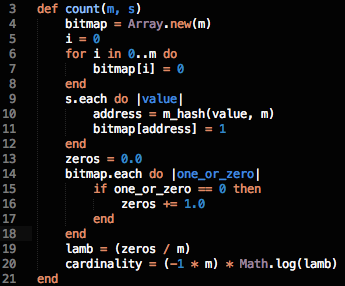
\includegraphics[scale=0.4]{fb_problem/lpc}
\caption{Determining the cardinality}
\end{framed}
\end{floatingfigure}
\noindent The Linear Probabilistic Counter algorithm also allows us to specify the amount of error we are willing to tolerate.
This is accomplished by changing the size of the bitmap; if the bitmap is large, or close to the size of the original set $\mathbb{S}$, then the error will be small.
Alternatively, if we decrease the size of the bitmap, we use less memory, but the error grows exponentially \cite{Hoff}.\\
\indent We can use the Linear Probabilistic Counter algorithm to solve the Facebook problem; unfortunately, we have no way of accessing the actual data we need, so we will have to do some guessing. 
We know that Facebook users make about 7,000,000 app installs a day \cite{Facebook-2}.
This means that the size of the set $\mathbb{S}$ will be 7,000,000.
Now we need to make some guesses; we expect that the applications that are most installed will appear a lot in our set, and that the applications that are installed less will appear less in $\mathbb{S}$. 
We do have access the to the top 20 Facebook application installs in August 2015, so we can plot those points and look for a trend in the data.
Doing so tells us that the data follows an exponential curve \cite{Facebook-2}, which means that Spotify (the top application at the time) will appear frequently in $\mathbb{S}$, whereas LINE, the $20^{\text{th}}$ most popular Facebook app, will appear sparingly.
This means that we will need a bitmap relatively close in size to the original set, since only a select few of the application have a high appearance rate in $\mathbb{S}$.
In other words, we expect a lot of distinct elements in $\mathbb{S}$.\\
\indent We can model the exponential function by choosing pseudo-random numbers weighted by a pre defined function.
We will let the each number correspond to a different application.
For example, if we let 200 be the number for Spotify, we would expect a high appearance rate of 200 in $\mathbb{S}$.
We can use an algorithm (courtesy of GitHub user Danieth5x) that will generate a pseudo-random sample based on a function, which will be an exponential function in our case.
We can argue that it is not important which exponential function we choose, since the distribution will be more or less the same; in our case we pick $e^{x}$.
Running the pseudo-random generator produces a set $\mathbb{S}$ of size 7,000,000, and we can now apply the Linear Probabilistic Counter to the data set.
For our purposes, we will use the hash function supplied by Ruby; the only change we need to make is to mod the result of the Ruby hash with the number of spaces in the bitmap, which ensures that we never produce a  hashed value out of the bounds of our bitmap.
Finally, running the algorithm tells us that the total number of unique application installs is 3216.\\

\indent The Linear Probabilistic Counter and the hash table algorithms handled relatively small data sets well, but the Twitter problem deals with a data set of nearly 200,000,000 tweets a day \cite{Twitter-2}.
The Linear Probabilistic Counter is too inefficient to process all the data, but the HyperLogLog algorithm allows for data to be processed more efficiently than the Linear Probabilistic Counter or the hash table. 
The HyperLogLog algorithm actually uses parts of the hash table and Linear Probabilistic Counter algorithms; values are still hashed to a bitmap held in memory. 
The hash function hashes values to binary numbers, and the algorithm decides whether that value has already been seen by analyzing the leading 0's in the binary number \cite[pp. 685, 689]{Heule}.
In other words, the algorithm keeps a record of the first location of a 1 in a binary string, called $\rho$ \cite[pp. 130]{Flaj}.
If the sequence of 0's is identical to another sequence of 0's, the probability that the original values were the same is very high, and the algorithm will ignore what it finds to be a duplicate value. 
The amount of memory that the HyperLogLog algorithm requires per bitmap is
\[
\text{Memory Required}\, = \log_{2}{\left(\log_{2}{\left(M \right)}\right)},
\]
where $M$ is the size of the original set of data \cite[pp. 129]{Flaj}.
The error amount is
\[
\text{Error}\ = \frac{\sqrt{3\log{(2)} - 1}}{\sqrt{m}},
\]
where $m$ is the number of spaces in the bitmap.
Finally, the algorithm takes the harmonic average of all the totals of the separate bitmaps, given by
\[
H = \frac{n}{\sum_{i=1}^{n}\frac{1}{x_{i}}},
\] 
which allows the algorithm to increase in accuracy as the size of the original set grows \cite{Yousra}.\\

\indent We can solve the Twitter problem with the HyperLogLog algorithm.
We use the code in \textit{Figure 3} to aggregate a random sampling of the most recent 2000 tweets that contain a ``\#'' every two minutes for 24 hours.
This allows for a large random sample of tweets that will closely model the real problem that we are trying to solve.
We also need a hashing function that will produce a binary string of 1's and 0's given any key; luckily this hash function already exists.
A murmur hash will produce a 32 bit binary string, which is exactly what we need.
Finally, we implement the algorithm. 
We create a class to perform the calculation that is initialized with the amount of memory we are willing to spend on the bitmap for the HyperLogLog algorithm. 
We know that the HyperLogLog can process nearly 1 billion elements with only 1.5 kilobytes of space to an accuracy of 2\% \cite{Flaj}.
%This estimate is given by the equation we have for memory.
Using a similar argument, we can determine the amount of memory we will need.
\begin{floatingfigure}[hr]{8cm}
\centering
\begin{framed}
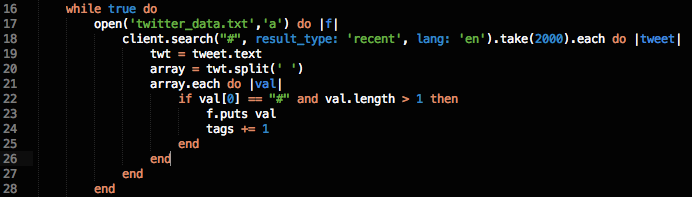
\includegraphics[scale=0.3]{Twitter_problem/ruby_code_01}
\caption{An infinite while loop can be useful}
\end{framed}
\end{floatingfigure}
\noindent If we want the error to be 1\%, then we calculate the number of spaces required in the bitmap by using the equation we have for the error.
\begin{align*}
0.01 &= \frac{\sqrt{3\log{(2)} - 1}}{\sqrt{m}}\\
m &= \frac{\sqrt{3\log{(2)} - 1}}{0.01^{2}}\\
m &\approx 10,794.4\ \text{spaces in the bitmap}.
\end{align*}
Now we can find the total memory required for our logarithm. If we let the program from \textit{Figure 3} run for 24 hours, at worst it will parse 1,440,000 hashtags.
We calculate the memory required by
\begin{align*}
\text{Memory}\, &= \log_{2}{(\log_{2}{(1,440,000)})}\\
&= 4.35457 \, \text{bytes per entry}.
\end{align*}
Multiplying this number by the total number of entires gives us a grand total of 47005 bytes, or 4.7005 kilobytes of required memory.\\

\indent We now have all the necessary information to parse the data. We implement the HyperLogLog in an object oriented manner; that is, we create a Ruby class called HyperLogLog that we initialize with the number of bytes per entry.
We also need a method to calculate the unique elements, and we need a way to call this routine.
\begin{center}
\begin{tabular}{c c c}
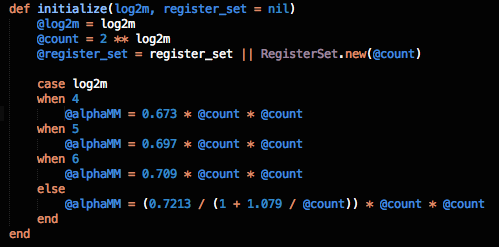
\includegraphics[scale=0.3]{Twitter_problem/hll_init}
&
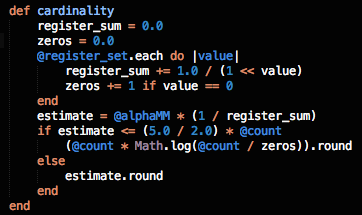
\includegraphics[scale=0.4]{Twitter_problem/hll_count}
&
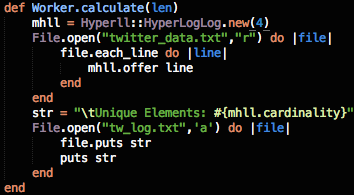
\includegraphics[scale=0.4]{Twitter_problem/hll_imp}
\\
Initialization & Counting & Implementing
\end{tabular}
\end{center}
\noindent \\
Note that we settled with 4 as the size of each entry in the bit-map. This value is close enough to 4.35 to say that the error will be just about 1\%.
Finally, in our main program, we loop infinitely (it will be up to us as to when to stop the program), and read in $\sim 2000$ tweets every two minutes. 
After running the algorithm for 24 hours, we will have a set of data that represents the number of unique hashtags found (by using the HyperLogLog algorithm) as the number of tweets being analyzed increases.
The data grow in a linear fashion; this is expected since we are gathering a random sample from all over the world, which means that at any given time, we expect to see about the same number of unique hashtags.
Plotting the data and applying a best fit line using Mathematica gives us
\[
f(x) = 0.284356 x + 7,361.39.
\]
From this data, we can make an estimate that at 200,000,000 tweets, we have
\begin{align*}
f(200,000,000) &= 0.284356(200,000,000) + 7,361.39\\
&= 56,878,500,
\end{align*}
which means that we have roughly 56 million unique hashtags by the HyperLogLog algorithm.\\ 

\indent We have looked at three different approaches to the count distinct problem. 
We used the HyperLogLog to solve only the Twitter problem, but we could have used the algorithm to solve all of the problems. 
The count distinct problem is widely applicable in the real world; companies are able analyze numbers that are determined by algorithms such as the HyperLogLog to increase profits, target ads, and keep more data.
An efficient way to count large sets of data may never be completely accurate. With algorithms like the HyperLogLog and the Linear Probabilistic counter, we can efficiently and with nearly 100\% accuracy solve the count distinct problem.

\newpage
\begin{thebibliography}{9}
\bibitem{Twitter} \#numbers. (2011, March 14). Retrieved October 29, 2015, from \url{https://blog.Twitter.com/2011/numbers}
\bibitem{SHA-Algo} Chaves, Ricardo, Kuzmanov, Georgi, Sousa, Leonel \& Vassiliadis, Stamatis (2006). Improving SHA-2 Hardware Implementations. , 4249, 298-310.
\bibitem{Facebook} Facebook Statistics. (2015, September 20). Retrieved October 30, 2015, from \url{http://www.statisticbrain.com/facebook-statistics/}
\bibitem{Flaj} Flajolet, P., Fusy, \'E., Gandouet, O., \& Meunier, F. (n.d.). HyperLogLog: The Analysis of a Near-Optimal Cardinality Estimation Algorithm. 2007 \textit{Conference on Analysis of Algorithms, 07,} 127-143. Retrieved October 27, 2015, from \url{http://algo.inria.fr/flajolet/Publications/FlFuGaMe07.pdf}
\bibitem{Heule} Heule, S., Nunkesser, M., \& Hall, A. (2013). HyperLogLog in Practice: Algorithmic Engineering of a State of the Art Cardinality Estimation Algorithm. In \textit{Proceedings of the 16th International Conference on Extending Database Technology} (Vol. EDBT '13, pp. 683-692). New York, NY, Genoa: ACM.
\bibitem{Hoff} Hoff, T. (2012, April 5). Big Data Counting: How to count a billion distinct objects using only 1.5KB of Memory - High Scalability -. Retrieved October 27, 2015, from \url{http://highscalability.com/blog/2012/4/5/big-data-counting-how-to-count-a-billion-distinct-objects-us.html}
\bibitem{Pokemon} How many Pokemon are there altogether, before and after Omega Ruby and Alpha Sapphire? (2014, October 27). Retrieved October 29, 2015, from \url{http://pokemondb.net/pokebase/219332/pokemon-there-altogether-before-after-omega-alpha-sapphire}
\bibitem{Maurer} Maurer, W. D. \& Lewis, T. G. (1975). Hash Table Methods. ACM Comput. Surv., 7, 5-19.
\bibitem{Facebook-2} Most popular Facebook apps 2015 | Statistic. (2015, August 1). Retrieved November 3, 2015, from \url{http://www.statista.com/statistics/276371/most-popular-facebook-apps-by-monthly-active-users/}
\bibitem{Twitter-2} Twitter Statistics. (2015, September 15). Retrieved November 3, 2015, from \url{http://www.statisticbrain.com/Twitter-statistics/}
\bibitem{Break-MD5} Wang, Xiaoyun \& Yu, Hongbo (2005). How to Break MD5 and Other Hash Functions. , 3494, 19-35.
\bibitem{Whang} Whang, Kyu-Young, Vander-Zanden, Brad T. \& Taylor, Howard M. (1990). A Linear-time Probabilistic Counting Algorithm for Database Applications. ACM Trans. Database Syst., 15, 208-229.
\bibitem{Yousra}Yousra Chabchoub, Georges H\'ebrail. \textit{Sliding HyperLogLog: Estimating cardinality in a data stream.} 2010. 
\end{thebibliography}
\end{document}